\documentclass[11pt,dvipsnames]{report} % {{{
\usepackage[spanish]{babel}
\usepackage[utf8]{inputenc}
\usepackage[T1]{fontenc}
\usepackage{makeidx}
\usepackage{graphicx}
\usepackage{subfig}
\usepackage{amsmath}
\usepackage{amsfonts}
\usepackage{amssymb}
\usepackage{authblk} % para la manipulación de autores y afiliación
\usepackage[pdftex]{hyperref}
\usepackage{multirow}
\usepackage{multicol}
\usepackage{float}
\usepackage{xcolor}
\usepackage{booktabs}
\usepackage{colortbl}
\usepackage{bbold}
\usepackage{physics}
\usepackage{mathtools}
\usepackage{dsfont}
\usepackage{tensor}

% Theorems, proofs, etc
\usepackage{amsthm}



\usepackage{fancybox}
\usepackage{colortbl}
\usepackage{amsbsy}
\usepackage[draft,inline,nomargin]{fixme} \fxsetup{theme=color}

%This defines my comments
\definecolor{mycolor}{RGB}{255,50,0}
\FXRegisterAuthor{ja}{aja}{\color{mycolor}JA}


\usepackage[]{lineno} \linenumbers
\setlength\linenumbersep{3pt}

\newcommand{\fref}[1]{fig.~\ref{#1}}  \newcommand{\tref}[1]{table~\ref{#1}}
\newcommand{\Fref}[1]{Fig.~\ref{#1}}  \newcommand{\Tref}[1]{Table~\ref{#1}}

\usepackage{hyperref}
%\usepackage{commath}
\decimalpoint
\renewcommand{\tablename}{Tabla}
\oddsidemargin 0in
\textwidth 6.5in
\topmargin -0.5in
\textheight 8.5in

\newcommand{\psii}{\psi_i}
\newcommand{\Pk}[1]{\ket{\psi_{#1} }}
\newcommand{\Pb}[1]{\bra{\psi_{#1} }}
\newcommand{\pk}{\ket{\psi}}
\newcommand{\M}{\mathcal{M}^{(N)}}
\newcommand{\E}{\mathcal{E}}
\newcommand{\Erho}{\mathcal{E}(\rho)}
\newcommand{\1}{\mathds{1}}
\newcommand{\ten}{\otimes}
\newcommand{\h}[1]{\colorbox{Yellow}{#1}}
\newcommand{\hi}{\mathcal{H}}
\newcommand{\txt}[1]{\text{#1}}
\newcommand{\here}{\h{\hspace{15cm}} }
\newcommand{\rhoi}{\dyad{\psii}{\psii}}
\newcommand{\ind}[2]{{{}^{#1}_{#2}}}
\newcommand{\QH}{\abs{Q_H}}
\newcommand{\QL}{\abs{Q_L}}
\newcommand{\W}{\abs{W}}
\newcommand{\uv}[1]{\vb{\hat{#1}}}
\newcommand{\ep}{\epsilon_0}

\def\dbar{{\mathchar'26\mkern-12mu d}}


% Para que funcione mejor la numeración {{{
% https://tex.stackexchange.com/questions/43648/why-doesnt-lineno-number-a-paragraph-when-it-is-followed-by-an-align-equation
\newcommand*\patchAmsMathEnvironmentForLineno[1]{%
  \expandafter\let\csname old#1\expandafter\endcsname\csname #1\endcsname
  \expandafter\let\csname oldend#1\expandafter\endcsname\csname end#1\endcsname
  \renewenvironment{#1}%
     {\linenomath\csname old#1\endcsname}%
     {\csname oldend#1\endcsname\endlinenomath}}% 
\newcommand*\patchBothAmsMathEnvironmentsForLineno[1]{%
  \patchAmsMathEnvironmentForLineno{#1}%
  \patchAmsMathEnvironmentForLineno{#1*}}%
\AtBeginDocument{%
\patchBothAmsMathEnvironmentsForLineno{equation}%
\patchBothAmsMathEnvironmentsForLineno{align}%
\patchBothAmsMathEnvironmentsForLineno{flalign}%
\patchBothAmsMathEnvironmentsForLineno{alignat}%
\patchBothAmsMathEnvironmentsForLineno{gather}%
\patchBothAmsMathEnvironmentsForLineno{multline}%
}
% }}}
% }}}
\title{Notas de estudio para Examen Privado\\
Licenciatura en Física}
\author{J.A. de León}

\newtheorem{definition}{Definición}[section]

\newtheorem{teorema}{Teorema}[section]

\newtheorem{property}{Propiedad}[section]

\begin{document}
\maketitle

\chapter{Termodinámica}
\section{Trabajo}
\begin{enumerate}
\item Durante un \textbf{proceso cuasiestático} un sistema atraviesa 
		en todo momento 
	  estados infinitesimalmente cercanos al equilibrio termodinámico y, 
	  por consiguiente, la dinámica de los estados puede ser descrita
	  en términos de coordenadas termodinámicas $\Rightarrow$ existe 
	  una ecuación de estado que describe estos estados 
\item Equilibrio termodinámico: eq. mecánico $+$ eq. térmico $+$ 
 	  eq. químico
\item Diferencial de trabajo de un sistema de un gas en un pistón:
\begin{equation}
\dbar W= PAdx = -PdV,
\end{equation}
el signo negativo asegura que en una compresión $(dV<0)$ $\dbar W>0$ 
(trabajo sobre el sistema, i.e. el sistema gana energía). 
\item El trabajo realizado sobre un sistema hidrostático depende de 
la trayectoria que se siga en el diagrama de estados (a diferencia
del trabajo realizado por la fuerza gravitacional, por ej). 
\item El trabajo relizado sobre un gas, definido por
\begin{align*}
W=-\int_{V_i}^{V_f} PdV, 
\end{align*}
se puede integrar siempre y cuando se conozca una función 
de estado.
\item ¡¡¡Calor $=$ energía!!!
\end{enumerate}

\section{1era ley de la Termodinámica}
\begin{itemize}
\item Una forma \textbf{restringida} de enunciar la primera ley 
de la termodinámica es:

Si un sistema cerrado es causado a cambiar de estado de un estado 
inicial a un estado final únicamente por procesos adiabáticos, entonces
el trabajo realizado sobre el sistema es el mismo para todas las trayectorias
adiabáticas que conectan a ambos estados. 

Es restringida porque no se está diciendo qué ocurre en 
aquellos procesos no adiabáticos. Es decir, en procesos
en los que ocurre intercambio de calor. 
\item Se sigue de esta forma restringida de la primera ley de la 
Termodinámica que existe una función que depende únicamente
de las coordenadas termodinámicas cuya diferencia entre el valor
final e inicial es igual al trabajo adiabático que se realiza al
sistema pasar del estado inicial al estado final. Esta función 
es la función de \textbf{energía interna} $U$: 
\begin{align}
W_{i\to f}\text{(adiabático)}=U_f-U_i,
\end{align}
esta diferencia da el aumento en energía interna del sistema. 
\item  \textbf{1era. ley de la Termodinámica} (formulación 
matemática): 
Cuando un sistema cerrado y su entorno se encuentran a distintas
temperatura y se realiza trabajo diatérmico [?] sobre el sistema,
entonces la energía transferida por otros procesos no mecánicos, 
igual a la diferencia entre el cambio de energía interna y el 
trabajo diatérmano se llama calor $Q$:
\begin{align}
  \Delta U = Q + W,
  \label{eq:1st-law-thermodynamics}
\end{align}
donde $Q>0$ cuando el calor entra al sistema y $Q<0$ cundo
abandona el sistema. Tres ideas están plasmadas en 
\eqref{eq:1st-law-thermodynamics}: (1) la existencia de una 
función de energía interna, (2) el principio de conservación de 
la energía, y (3) la definición de trabajo como energía en tránsito
en virtud de una diferencia de temperatura.
\item \textbf{Forma diferencial de la 1era. ley de la Termodinámica}:
para un sistema termodinámico que atraviesa cambios infinitesimales 
en sus variables termodinámicas la primera ley se formula como
\begin{align}
  dU = \dbar Q + \dbar W.
  \label{eq:1st-law-thermodynamics_diffForm}
\end{align}
\item \textbf{Capacidad calorífica}: 
\begin{align}
  C=\dv{Q}{T} \qty[\frac{K}{J}]
  \label{eq:heat-capacity}.
\end{align}
\item El caso de un gas:

La ecuación \eqref{eq:1st-law-thermodynamics_diffForm} toma 
la forma 
\begin{align}
   dU =\dbar Q-PdV,
   \label{eq:1st-law-gas}
 \end{align} 
donde $U$ es una función de algún par $P,V,T$ (la ecuación relaciona 
a un par con la tercera). Tomando $U=U(T,V)$ se tiene 
\begin{align*}
dU=\qty(\pdv{U}{T	})_VdT+\qty(\pdv{U}{V})_TdV,
\end{align*}
y sustityendo en \eqref{eq:1st-law-gas}
\begin{align*}
\dbar Q &=\qty(\pdv{U}{T	})_VdT+\qty[\qty(\pdv{U}{V})_T+P]dV\\
\dv{Q}{T} &= \qty(\pdv{U}{T	})_V
+\qty[\qty(\pdv{U}{V})_T+P]\dv{V}{T}.
\end{align*}
\item Flujo cuasiestático de calor: cuando a lo largo de un sistema 
existe un gradiente de temperatura y el calor fluye de manera
cuasiestática (misma definición) podemos calcular el 
calor que se absorbe durante el proceso utilizando la ecuación 
\eqref{eq:heat-capacity} de la capacidad calorífica.
\item El transporte de energía en un sistema entre elementos
de volumen vecinos en virtud de una diferencia de temperatura se 
conoce como conducción de calor. Los experimentos muestran que 
\begin{align*}
\frac{Q}{t}\propto A\frac{\Delta T}{\Delta x},
\end{align*}
con $A$ el área transversal al flujo de calor. Por consiguiente
\begin{align}
\dv{Q}{t	} = -KA\dv{T}{x},
\end{align}
con $K$ la conductividad térmica. El signo menos es para asegurar
que la dirección del flujo de calor sea en la dirección positiva de $x$.
\item \textbf{Radiación térmica}: radiación en virtud de su temperatura.
\item Exitancia radiante $\mathcal{R}$: potencia irradiada total por 
unidad de área. Emisividad total $\epsilon$: fracción de la potencia
irradiada total que es emitida como radiación térmica.
\item \textbf{Ley de Stefan-Boltzmann}: un cuerpo negro es una
sustancia ideal que es capaz de absorber toda la luz incidente 
sobre ella y reemitirla netamente como radiación térmica. La
radiación de un cuerpo como este está dada por la la siguiente ley:
\begin{align}
  \mathcal{R}=\mathcal{R}(T)=\sigma T^4,
  \label{eq:stefan-boltzmann}
\end{align}
donde $\sigma$ es la constante de Stefan-Boltzmann.
\end{itemize}

\section{Gas ideal}
\begin{enumerate}
\item \textbf{Expansión libre adiabática}: gas en expansión en el 
cual no se hace trabajo ni se transfiere calor $\Rightarrow$ $\Delta U=0$
durante la expansión libre.
\item Al escribir explícitamente $dU$ asumiendo que $U=U(T,V)$ ó 
$U=U(T,P)$ y al considerar una expansión libre adiabática $(dU=0)$
se concluye que $U=U(T)$ para un gas ideal. 
\item Un \textbf{gas ideal} satisface
\begin{align}
  PV&=nRT, & \qty(\pdv{U}{P})_T&=0,
  \label{eq:ideal-gas}
\end{align}
la primera condición es la ecuación de estado del gas ideal y 
la segunda es para asegurar que en una expansión libre
$dU=0$.
\item Retomando la ecuación \eqref{eq:1st-law-gas}:
\begin{align*}
\dbar Q=dU+PdV,
\end{align*}
cuando $dV=0$
\begin{align*}
\qty(\dv{Q}{T})_T=C_V=\qty(\pdv{U}{T})_V.
\end{align*}
En el caso del gas ideal $U=U(T)$, por consiguiente
\begin{align*}
C_V=\dv{U}{T},
\end{align*}
y 
\begin{align*}
\dbar Q = C_VdT+PdV,
\end{align*}
y sacando un diferencial de la ecuación de estado del gas ideal
\begin{align*}
PdV+VdP=nRdT.
\end{align*}
Sustiyendo arriba
\begin{align*}
\dbar Q &= C_VdT + nRdT - VdP\\
\dv{Q}{T}&=\qty(C_V+nR)-V\dv{P}{T},
\end{align*}
cuando $dP=0$:
\begin{align}
  \qty(\dv{Q}{T})_P=C_P=C_V+nR.
  \label{eq:C_P-idealGas}
\end{align}
\end{enumerate}




































\chapter{Mecánica Estadística}


\section{Fundamentos estadísticos de la Termodinámica}
\begin{itemize}
	\item La especificación de los valores de los parámetros $N$, $V$ y $E$
	define a un \textbf{macroestado}.
	
	\item Los \textbf{microestados} se identifican como las posibles 
	configuraciones de un sistema para dar lugar al mismo valor 
	de energía $E$ del sistema completo, $\Omega=\Omega(N,V,E).$
	
	\item \textbf{Postulado de la igualdad de probabilidad apriori:} el sistema
	tiene igualdad de probabilidad de estar en cualquiera de los posibles
	microestados.
	
	\item Al colocar dos sistemas termodinámicos en contacto se supone
	que estos llegarán al equilibrio cuando se el valor de la energía
	del sistema (\janote{del sistema?}) maximice el número 
	de microestados en los que se puede encontrar el sistema.
	El macroestado con la mayor cantidad de microestados 
	se dice que es el más probable.
	
	\item $S=k\ln \Omega$: entropía absoluta en términos del número
	total de microestados accesibles según el macroestado del sistema.
	
	\item De la fórmula que enunció Planck sobre la entropía (ya había
	sido formulada por Boltzmann, pero fue Planck quien la escribió en la
	forma moderna) se desprende que la entropía se hace cero cuando 
	el sistema puede encontrarse en una sola configuración.
	
	\item \textbf{El gas ideal clásico}: dado que asumimos que las 
	partículas no interactúan entre sí dentro del gas, entonces
	\begin{align}
	\Omega (N,E,V)\propto V^N,
	\end{align}
	y esto nos lleva a que 
	\begin{align}
	\pdv{S}{V}&=\frac{P}{T}=k\qty(\pdv{\ln \Omega \qty(N,E,V)}{V})_{N,E}=
	k\frac{N}{V}  \\
	PV&=kNT = nRT \hspace{1.5cm} (R=kN_A),
	\end{align}
	así hemos llegado a la ecuación de estado del gas ideal desde 
	principios estadísticos.
	
	\item \textbf{Paradoja de Gibbs (entropía de mezcla):} Gibbs consideró
	una situación como la de la \Fref{fig:gibbs-paradox} en la que 2 gases
	iguales se mantienen a ambos lados de una pared diatérmana, luego
	la pared se quita y se permite que ambos gases se mezclen. En este 
	caso particular tenemos un proceso reversible porque podemos 
	volver a colocar la pared y tendríamos la misma situación inicial. 
	Sin embargo, con métodos estadísticos se concluye que la diferencia
	de entropía entre los estados inicial y final del sistema total es distinto
	de cero, lo que contradice lo bien conocido de la termodinámica 
	de que en un proceso reversible adiabático el cambio en la 
	entropía es igual a cero. La propuesta de Gibbs para resolver
	esta paradoja fue cambiar la expresión de la entropía $S$ de 
	un gas ideal de 
	\begin{align}
	S(N,V,E)=Nk\ln\qty[\frac{V}{h^3}\qty(\frac{4\pi mE}{3N})^{3/2}]
	+\frac{3}{2}Nk
	\end{align}
	a
	\begin{align}
	S(N,V,E)=Nk\ln\qty[\frac{V}{Nh^3}\qty(\frac{4\pi mE}{N})^{3/2}]
	+\frac{5}{2}Nk,
	\end{align}
	habiendo así agregado de manera \textit{ad hoc} los términos
	$-k\ln N!$ $(\approx Nk\ln N-Nk)$.
	\begin{figure}
	    \centering
	    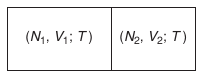
\includegraphics[width=5cm]{images/mixing-2gases.png}
	    \caption{Mezcla de dos gases ideales.}
	    \label{fig:gibbs-paradox}
	  \end{figure}
	  
	\item La consecuencia física del arreglo de Gibbs es que se está 
	reduciendo el número de microestados accesibles por el sistema 
	en un factor $N!$. La justificación de esto es que estamos lidiando
  con partículas idénticas que son indistinguibles, por consiguiente
  no tiene sentido etiquetar individualmente a cada una de las
  partículas. Todo lo que podemos contar es la distribución 
  sobre los estados de energía.
\end{itemize}

\section{Elementos de la teoría de los ensambles}
\begin{itemize}
	\item Un microestado de un sistema clásico, en un tiempo $t$, está
	definido por las posiciones y momenta de todas las partículas
	que constituyen al sistema.
	\item Las coordenadas $(q_i,p_i)$ representan un punto en 
	un espacio de $6N$ dimensiones conocido como el espacio de fases.
	\item Función de densidad $\rho(q,p;t)$: para describir mejor 
	los ensambles de microestados en los que se puede encontrar
	un sistema. Esta función es tal que el número de puntos 
	representativos dentro del elemento de volumen $d^{3N}qd^{3N}p$
	alrededor del punto $(q,p)$ del espacio de fases está dado por 
	el proudcto $\rho(q,p;t)d^{3N}qd^{3N}p$.
	\item El promedio del ensamble $\expval{f}$ de una cantidad
	física $f(q,p)$ está dado por 
	\begin{align}
	\expval{f}=
	\frac{\int f(q,p)\rho(q,p;t)d^{3N}qd^{3N}p}{\int \rho(q,p;t)d^{3N}qd^{3N}p}
	\end{align}
	
	\item \textbf{Teorema de Liouville:} Consideremos una región de
	volumen arbitrario $\omega$, cuya superficie la vamos a denotar
	por $\sigma$, como se ve en la \Fref{fig:liouville}. 
	Entonces, la tasa a la que el número de puntos 
	representativos en este elemento de volumen aumenta con 
	el tiempo es
	\begin{align}
	\pdv{t}\int_{\omega} \rho d\omega.
	\end{align}
	Por otro lado, el flujo hacia afuera de $\omega$ está dado por 
	\begin{align}
	\int _{\sigma}\rho \vb{v}\cdot \vb{\hat{n}}d\sigma.
	\end{align}
	Por el teorema de la divergencia (que no tengo fresco en el momento
	que estoy escribiendo esto \janote{OJO}) tenemos 
	\begin{align}
	\int _\omega \div{\rho \vb{v}}d\omega.
	\end{align}
	En vista que no hay fuentes ni sumideros
	\begin{align}
	\pdv{t}\int_{\omega} \rho d\omega=-\int _\omega \div{\rho \vb{v}}d\omega,
	\end{align}
	por lo que 
	\begin{align}
	\int _{\omega}\qty(\pdv{\rho}{t}+\div{\rho\vb{v}})d\omega=0.
	\end{align}
	Por lo cual, inmediatamente se tiene 
	\begin{align}
	\pdv{\rho}{t}+\div{\rho\vb{v}}=0,
	\end{align}
	y esta ecuación es conocida como la ecuación de continuidad. 
	Trabajando más esta ecuación 
	\begin{align}
	\pdv{\rho}{t}+\sum_{i=1}^{3N}
	\qty(\pdv{\rho}{q_i}\dot{q}_i+\pdv{\rho}{p_i}\dot{p}_i)+
	\rho \sum_{i=1}^{3N}
	\qty(\pdv{\dot{q}_i}{q_i} + \pdv{\dot{p}_i}{p_i})=0.
	\end{align}
	\h{Recordatorio eqs. de Hamilton:} 
	\begin{align}
	\dot{q}_i&=\pdv{H(q_i,p_i)}{p_i}\\
	\dot{p}_i&=-\pdv{H(q_i,p_i)}{q_i}.
	\end{align}
	Usando la ecuaciones de Hamilton notamos que 
	el tercer término en la ecuación de continuidad se hace cero,
	por consiguiente llegamos al resultado 
	conocido como el \h{teorema de Liouville}:
	\begin{align}
	\pdv{\rho}{t}+\{\rho,H\}=0,
	\end{align}
	donde $\{\rho,H\}$ es el bracket de Poisson. La consecuencia 
	física de este teorema es que las trayectorias en el espacio de 
	fases se mueven de la misma manera que un fluido 
	incompresible.
	\begin{figure}
	  \centering
	  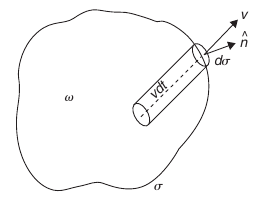
\includegraphics[width=5cm]{images/phase-space.png}
	  \caption{Elemento de volumen en el espacio de fases.}
	  \label{fig:liouville}
	\end{figure}
	
	\item \textbf{Ensamble canónico:} $E=$ cte.
	
	\item \textbf{El ensamble microcanónico:}
	El macroestado del ensamble microcanónico de un sistema está 
	definido por el número de moléculas $N$, el volumen $V$ y la 
	energía $E$. El ensamble microcanónico es una colección de
	sistemas para los cuales la función de densidad $\rho$ está 
	dada por 
	\begin{align}
	\rho(q,p)=\text{cte.}\hspace{1cm}
	\text{si} \hspace{2mm}
	\qty(E-\frac{1}{2}\Delta)\leq
	H(q,p)\leq
	\qty(E+\frac{1}{2}\Delta).
	\end{align}
	
	\item El resultado fundamental es llegar a la \textbf{energía 
	libre de Helmholtz!!!!} (ver sec. 3.3 Pathria)
	
	\item El formalismo del ensamble microcanónico y canónico son equivalentes.
	
	\item \textbf{Teorema de equipartición:} (revisar notas en Drive para la 
	deducción matemática) cada término armónico en el Hamiltoniano 
	transformado de un sistema contribuye $1/2kT$ a la energía 
	interna del sistema. Dicho de otro modo, cada grado de libertad 
	aporta la misma cantidad al valor esperado de la energía del sistema 
	total. \textbf{No obstante}, el teorema de equipartición es válido 
	para valores de temperatura muy altos, osea cuando los 
	grados de libertad relevantes del sistema pueden 
	ser excitados libremente.
	
	\item \textbf{Teorema del virial:} (revisar notas en Driva para la 
	deducción) 
	\begin{align}
	-\expval{\sum_iq_i\dot{p_i}}=3NkT,
	\end{align}
	donde
	\begin{align}
	\mathcal{V}=-3NkT,
	\end{align}
	es	llamado el 'virial' del sistema.
	Cuando se considera a un gas ideal esto se reduce a la relación 
	clásica:
	\begin{align}
	\mathcal{V}=-2K,
	\end{align}
	con $K$ la energía cinética del sistema.	
\end{itemize}

\subsection{Osciladores armónicos}
Asumiendo osciladores armónicos en una dimensión el hamiltoniano
$H$ del sistema es 
\begin{align}
H(q_i,p_i)=\sum_i\frac{1}{2}m\omega^2q_i^2+\frac{1}{2m}p_i^2.
\end{align}
Al calcular la función de partición $\mathcal{Z}$ de un oscilador armónico
\begin{align}
\mathcal{Z}&=\int _{-\infty}^{\infty}\int _{-\infty}^{\infty}
\exp\qty[-\beta\qty(\frac{1}{2}m\omega^2q^2+\frac{1}{2m}p^2)]
\frac{dqdp}{h}\nonumber\\
&=\frac{1}{h}\qty(\frac{2\pi}{\beta m\omega^2})^{1/2}
\qty(\frac{2\pi m}{\beta})^{1/2}=
\frac{1}{\beta\hbar\omega}=\frac{kT}{\hbar\omega}.
\end{align}
De manera que entonces la función de partición del sistema 
completo es 
\begin{align}
\mathcal{Z}=\qty(\frac{kT}{\hbar\omega})^N.
\end{align}
La energía libre de Helmholtz está dada por 
\begin{align}
A&=-kT\ln \mathcal{Z}\nonumber\\
&=-NkT\ln\qty(\frac{kT}{\hbar\omega}).
\end{align}
De manera que las otras variables termodinámicas son
\begin{align}
S&=-\qty(\pdv{A}{T})_{N,V}\nonumber\\
&=Nk\qty[\ln\qty(\frac{kT}{\hbar\omega})+1]
\end{align}
y 
\begin{align}
U&=\pdv{\ln\mathcal{Z}}{\beta}\nonumber\\
&=NkT.
\end{align}
\chapter{Electromagnetismo}
\section{Electrostática}
\subsection{Campo eléctrico y ley de Gauss}
\begin{itemize}
\item El campo eléctrico producido por una densidad de carga $\rho(\vb{r})$
es
\begin{align}
\frac{q}{4\pi \epsilon_0}\int \frac{\rho(\vb{r}')}{r^2}\uv{r}dV'.
\end{align}

\item Se define el flujo de campo eléctrico $\vb{E}$ a través de 
una superficie $\mathcal{S}$ como
\begin{align}
\Phi_E\equiv\int _{\mathcal{S}}\vb{E}\vdot d\vb{a}.
\end{align}

\item \textbf{Ley de Gauss:}
\begin{align}
\oint \vb{E}\vdot d\vb{a}=\frac{1}{\ep}q_{\text{enc}},
\end{align}
el flujo de campo eléctrico atravesando una superficie cerrada
es proporcional a la carga que se encuentra encerrada dentro 
de la superficie. La dirección del flujo nos indica si tenemos un 
sumidero o una fuente y, al mismo tiempo, el signo de la carga
encerrada.

\item Es importante aprender a pasar de la forma integral, a la forma
diferencial de la ley de Gauss. Veamos a continuación. 
\begin{align*}
\oint_{\mathcal{S}} \vb{E}\vdot d\vb{a}=\int_{\mathcal{V}}
\qty(\div{\vb{E}})dV
\end{align*}
\textit{\textbf{Paréntesis (teorema de la divergencia)}: la integral 
de superficie cerrada de un campo vectorial es igual a la integral 
de volumen de la divergencia del campo vectorial, integrado sobre
el volumen que encierra la superficie,}

Recordando que 
\begin{align*}
q_{\text{enc}}&=\int_{\mathcal{V}}\rho \ dV,
\end{align*}
por consiguiente, 
\begin{align*}
\int_{\mathcal{V}}\qty(\div{\vb{E}})dV=
\frac{1}{\ep}\int_{\mathcal{V}}\rho \ dV,
\end{align*}
puesto que la integración es sobre el mismo volumen, entonces
los integrandos deben ser iguales,
\begin{align}
\div{\vb{E}}=\frac{\rho}{\ep}.
\end{align}

La ley de Gauss es siempre cierta, \textit{pero no siempre útil}.
Particularmente, las simetrías son cruciales para poder aprovechar 
el resultado establecido en la ley de Gauss:
\begin{enumerate}
\item Simetría esférica: superficie gaussiana una esfera concéntrica.
\item Simetría cilíndrica: superficie gaussiana un cilindro coaxial. 
\item Simetría plana: superficie gaussiana una caja de pastillas.
\end{enumerate}
Aprovecharse de las simetrías $+$ utilizar el principio de superposición
hace que la ley de Gauss se vuelva especialmente útil para su aplicación.

\item $\curl{\vb{E}}=0$. Tomemos el caso de una carga puntual
$q$, cuyo campo eléctrico $E$ es
\begin{align}
\vb{E}=\frac{1}{4\pi\ep}\frac{q}{r^2}\uv{r}.
\end{align}
Ahora calculemos la integral de línea entre dos puntos arbitrarios
$a$ y $b$ del espacio, 
\begin{align*}
\int_a^b \vb{E}\vdot d\vb{l}.
\end{align*}
En coordenadas esféricas, $d\vb{l}=dr\uv{r}
+rd\theta \uv{\boldsymbol{\theta}}+
r\sin\theta d\phi \uv{\boldsymbol{\phi}}$, entonces
\begin{align*}
\int_a^b\vb{E}\vdot d\vb{l}&=\int_a^b\frac{1}{4\pi\ep}\frac{q}{r^2}dr\\
&=\frac{q}{4\pi\ep}\qty(\frac{1}{r_a}-\frac{1}{r_b}),
\end{align*}
por lo tanto, al integrar sobre una trayectoria cerrada la integral 
debe ser igual a cero:
\begin{align}
\oint\vb{E}\vdot d\vb{l}=0.
\end{align}
Por consiguiente, aplicando el teorema de Stokes:
\begin{align}
\oint\vb{E}\vdot d\vb{l}&=\int \qty(\curl{\vb{E}})\vdot d\vb{a}=0\\
\therefore \hspace{5mm} \curl{\vb{E}}&=0.
\end{align}
Este resultado se sigue satisfaciendo para cualquier distribución 
estática de cargas, pues si tenemos $N$ cargas, el campo eléctrico
de la distribución está determinado por 
\begin{align*}
\vb{E}=\vb{E}_1+\vb{E}_2+\ldots+\vb{E}_N\\
\end{align*}
\begin{align}
\therefore \hspace{5mm} 
\curl{\vb{E}}=\curl{\vb{E}_1}+\curl{\vb{E}_2}+\ldots+
\curl{\vb{E}_N}=0,
\end{align}
dado que cada rotor se debe hacer cero.
\end{itemize}
\subsection{Potencial eléctrico}
\begin{itemize}
\item El \textbf{potencial eléctrico} es una función escalar que se define
como
\begin{align}
V(\vb{r})\equiv -\int_{\mathcal{O}}^r\vb{E}\vdot d\vb{l},
\end{align}
con $\mathcal{O}$ un punto de referencia.

\item El teorema fundamental de los gradientes establece que
\begin{align*}
V(\vb{r}_b)-V(\vb{r}_a)=\int_a^b \grad V\vdot d\vb{l},
\end{align*}
por consiguiente, 
\begin{align*}
\int_a^b \grad V\vdot d\vb{l}&=-\int_a^b \vb{E}\vdot d\vb{l}\\
\vb{E}&=-\grad V.
\end{align*}

\item Es una consecuencia de $\curl{\vb{E}}=0$ que las componentes
$E_i$ de $\vb{E}$ no sean completamente independientes entre ellas.
De hecho, la formulación del potencial eléctrico explota al máximo 
esto.

\item \textbf{Ecuación de Poisson:}
\begin{align}
\grad^2V=\frac{\rho}{\ep}.
\end{align}

\item Cálculo del potencial eléctrico $V$ a partir de la distribución de
carga $\rho$:
\begin{align}
\frac{1}{4\pi\ep}\int\frac{\rho(\vb{r}')}{r}\ dV'.
\end{align}

\item \textbf{Discontinuidad al cruzar una superficie de carga $\sigma$}:
supongamos una superficie con densidad superficial de cargar $\sigma$.
Consideremos un área $A$ sobre la superficie, tan pequeña como 
sea necesario para que $\sigma=\text{cte.}$, y apliquemos 
la ley de Gauss con una caja de pastillas gaussiana. Los lados 
de la caja de pastillas (componente paralela a la superficie) no 
contribuyen nada al flujo neto de campo eléctrico, por lo tanto, 
sumando las contribuciones perpendiculares a la superficie se 
tiene $\qty(E_{\text{arriba}}-E_{\text{abajo}})A=\sigma A/\ep$,
entonces $E_{\text{arriba}}-E_{\text{abajo}}=\sigma /\ep$. Por 
lo cual, se concluye que existe una discontinuidad de la componente 
normal de $\vb{E}$ al atravesar una superficie de carga que es igual 
a $\sigma/\ep$. Las componentes paralelas a la superficie son continuas
y es consecuencia directa de 
\begin{align}
\oint \vb{E}\vdot d\vb{l}=0.
\end{align}
No obstante, el potencial eléctrico es continuo a través de cualquier
frontera, ya que 
\begin{align*}
V_{\text{arriba}}-V_{\text{abajo}}=-\int_a^b\vb{E}\vdot d\vb{l};
\end{align*}
conforme la trayectoria entre $a$ y $b$ se hace igual a cero, 
también lo hace el valor de la integral, por consiguiente
\begin{align}
V_{\text{arriba}}=V_{\text{abajo}}.
\end{align}
\end{itemize}

\subsection{Trabajo y energía}
\begin{itemize}
\item De lo que sabemos de mecánica el trabajo sobre un sistema 
para moverlo desde $a$ hasta $b$ es 
\begin{align}
W=\int_a^b\vb{F}\vdot d\vb{l}.
\end{align}
Por consiguiente, el trabajo para mover una carga $q$ es
\begin{align}
W=-q\int_a^b\vb{E}\vdot d\vb{l}=q\qty(V_b-V_a)
\end{align}

\item La energía de una configuración de cargas se define 
como la cantidad de trabajo necesario para armar la configuración:
\begin{align}
W=\frac{1}{2}\sum_i^nq_iV(\vb{r}_i),
\label{eq:ch3-W-point}
\end{align}
donde $V$ es el potencial generado por el resto de las cargas 
en la configuración.

\item Si en vez tenemos una distribución continua de carga $\rho$
entonces podemos reescribir la ecuación \eqref{eq:ch3-W-point}
como
\begin{align}
W=\frac{1}{2} \int \rho Vd\tau.
\end{align}
Si utilizamos la ley de Gauss podemos resscribir esta ecuación como
\begin{align}
W&=\frac{\ep}{2} \int \qty(\div{\vb{E}}) Vd\tau\nonumber\\
&=\frac{\ep}{2}\qty(-\int \vb{E}\vdot \qty(\grad V)d\tau
+\oint V\vb{E}\vdot d\vb{a}),
\end{align}
pero como $\grad V=-\vb{E}$,
\begin{align}
W&=\frac{\ep}{2}\qty(\int E^2d\tau+\oint V\vb{E}\vdot d\vb{a}),
\end{align}
consideramos la integración sobre todo el espacio, y de esa manera,
\begin{align}
W&=\frac{\ep}{2}\int E^2d\tau.
\end{align}
\end{itemize}

\section{Potenciales}
\subsection{El método de imágenes}
\textbf{El problema:} supongamos una carga $q$ que se encuentra a 
una distancia $d$ sobre un plano conductor infinito, ¿cuál es el potencial
en una región por encima del plano?

El punto es establecer cuáles son las condiciones de frontera del problema
y luego encontrar una configuración equivalente que satisfaga dichas 
condiciones de frontera, de esa manera, justificados en el teorema de 
unicidad de las ecuaciones diferenciales, habremos encontrado 
la solución al problema. 

\section{Desplazamiento eléctrico}
\begin{itemize}
\item El efecto de la polarización es producir acumulaciones de carga 
$\rho_b=-\div{\vb{P}}$ dentro del dieléctrico y $\sigma_b=\vb{P}
\vdot \vb{\hat{n}}$ en la superficie. El campo eléctrico debido a la
polarización del medio es justo el campo generado 
por la carga ligada más la carga libre. 
\item Dentro de un dieléctrico, la densidad total de carga 
puede escribirse como 
\begin{align}
\rho=\rho_b+\rho_f,
\end{align}
y, entonces aplicando la ley de Gauss, tenemos 
\begin{align}
\ep \div{\vb{E}}=\rho=\rho_b+\rho_f=-\div{P}+\rho_f,
\end{align}
donde $\vb{E}$ es el campo total.
\begin{align}
\div{\qty(\ep \vb{E}+\vb{P})}=\rho_f.
\end{align}
Así definimos
\begin{align}
\vb{D} \equiv \qty(\ep \vb{E}+\vb{P}),
\end{align}
que se conoce como \textbf{desplazamiento eléctrico}. Por consiguiente, 
en términos de $\vb{D}$ la ley de Gauss se escribe como
\begin{align}
\div{\vb{D}}=\rho_f.
\end{align}
Esta forma de escribir a la ley de Gauss para dieléctricos es particularmente
útil porque solamente considera a la densidad de carga libre.
\item A diferencia del vector de campo eléctrico $\vb{E}$, la componente
paralela a una superficie conductora es discontinua, 
\begin{align}
\vb{D}^{\parallel}_{\text{arriba}}-\vb{D}^{\parallel}_{\text{abajo}}=
\vb{P}^{\parallel}_{\text{arriba}}-\vb{P}^{\parallel}_{\text{abajo}}.
\end{align}
\end{itemize}

\subsection{Dieléctricos lineales}
\begin{itemize}
\item Para muchos sistemas físicos la polarización $\vb{P}$ es directamente 
proporcional al campo eléctrico $\vb{E}$:
\begin{align}
\vb{P}=\ep \chi_e\vb{E},
\end{align}
con $\chi_e$ la susceptibilidad eléctrica del medio, depende 
de la estructura microscópica del medio.

\item En un medio lineal:
\begin{align}
\vb{D}=\ep\vb{E}+\vb{P}=\ep\vb{E}+\ep\chi_e\vb{E}=
\ep\qty(1+\chi_e)\vb{E},
\end{align}
entonces definimos
\begin{align}
\epsilon \equiv  \ep\qty(1+\chi_e).
\end{align}
Por lo tanto,
\begin{align*}
\vb{D}=\epsilon\vb{E}.
\end{align*}
\end{itemize}

\section{Magnetostática}
\subsection{Ley de Biot-Savart}
La electrostática y magnetostática ocurre cuando
\begin{align*}
\pdv{\rho}{t}=0, \hspace{3mm} \pdv{\vb{J}}{t}=0.
\end{align*}
(cargas y corrientes estacionarias.)

\begin{itemize}
\item \textbf{Ley de Biot-Savart} para corrientes estacionarias:
\begin{align}
\vb{B}(\vb{r})=\frac{\mu_0}{4\pi}I\int \frac{d\vb{l}'\cp\vb{\hat{r}}}
{r^2}
\end{align},
donde la integración se realiza a lo largo de trayectoria de la corriente
en la dirección del flujo $d\vb{l}'$.
\begin{align}
\qty[\tx{B}]=\frac{\tx{N}}{\tx{A}\cdot \tx{m}}=\tx{T}.
\end{align}

\item De acuerdo con la ley de Biot-Savart el campo magnético 
alredor de un cable infinito de corriente es 
\begin{align}
\vb{B}=\frac{\mu_0I}{2\pi s} \uv{\phi}.
\end{align}
De primera vista es evidente que $\curl{\vb{B}}\neq 0$,
\begin{align}
\oint \vb{B}\vdot d\vb{l}
= \oint\frac{\mu_0I}{2\pi s}\ dl =\mu_0 I.
\end{align}
Ahora si suponemos que tenemos un manojo de cables de 
corriente, cada uno contribuyendo $\mu_0I$ a la integral de 
$\vb{B}$ alrededor del manojo de cables, entonces la integral 
daría como resultado 
\begin{align*}
\oint \vb{B}\vdot d\vb{l}=\mu_0I_{\tx{enc}},
\label{eq:ampere-inc-law}
\end{align*}
donde $I_\tx{enc}$ es la corriente que encierra una espira 
alrededor de la corriente. También podemos escribir a la corriente
$I$ en términos de la densidad de corriente $\vb{J}$,
\begin{align}
I_{\tx{enc}}=\int \vb{J}\vdot d\vb{a}.
\end{align}
Si aplicamos el teorema de Stokes a la ecuación \eqref{eq:ampere-inc-law}
tenemos
\begin{align}
\int\curl{\vb{B}}\vdot d\vb{a}&=\mu_0\int \vb{J}\vdot d\vb{a}\\
\therefore \hspace{5mm} \curl{\vb{B}}&=\mu_0\vb{J}.
\end{align}
Esta es conocida como la ley de Ampère en forma diferencial.

\item \h{Revisar deducción formal de que la ley de Ampère se cumple 
para cualquier forma de $\vb{J}$,	} \newline
\h{siempre y cuando se cumpla $\div{\vb{J}}=0$.}

\item Similarmente a la ley de Gauss para campos eléctricos, la 
ley de Ampère es útil sólo cuando existen ciertas simetrías:
\begin{enumerate}
\item Líneas infinitas de corriente
\item Planos infinitos
\item Solenoides infinitos
\item Toroides
\end{enumerate}
\end{itemize}

\subsection{Vector potencial magnético}
Que se cumpla que $\div{\vb{B}}$ hace que exista una función 
vectorial de potencial $\vb{A}$ en magnetostática, tal que 
\begin{align}
\vb{B}=\curl{\vb{A}}.
\end{align}
Entonces
\begin{align}
\curl{\vb{B}}=\curl{\curl{\vb{A}}}=\grad{\qty(\div{\vb{A}})}
-\grad^2\vb{A}=\mu_0\vb{J}.
\end{align}
Si imponemos la condición de $\div{\vb{A}}=0$, entonces tenemos 
\begin{align}
\grad^2\vb{A}=-\mu_0\vb{J}.
\label{•}
\end{align}
Esta es simplementa la ecuación de Poisson, cuya solución, 
asumiendo que $\lim_{x\to\infty}\vb{J}=0$,
\begin{align}
\vb{A}(\vb{r})=\frac{\mu_0}{4\pi}\int \frac{\vb{J}(\vb{r}')}{r}\ dV'
\label{}
\end{align}
\subsection{Condiciones de frontera}
\begin{figure}
  \centering
  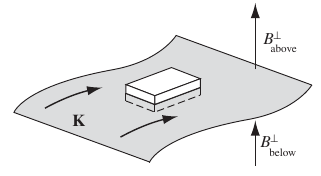
\includegraphics[width=6cm]{images/sup-current.png}
  \caption{Superficie de corriente.}
  \label{fig:sup-current}
\end{figure}
Si consideramos la situación en la \Fref{fig:sup-current} y recordamos que
$\div{\vb{B}}=0$, integramos sobre el volumen de la caja de pastillas,
y aplicamos el teorema de la diverencia 
\begin{align}
\oint \vb{B}\vdot d\vb{a}&=0\\
\qty(B^{\perp}_{\tx{arriba}}-B^{\perp}_{\tx{abajo}})A&=0\\
B^{\perp}_{\tx{arriba}}&=B^{\perp}_{\tx{abajo}}.
\end{align}
Si ahora tomamos una espira, digamos alrededor de una de las caras
de la caja de pastillas y hacemos que la altura de la caja sea 
infinitesimalmente pequeña, tanto como lo necesitemos para 
despreciar la contribución de la componente perpendicular 
del campo magnético, 
\begin{align}
\oint \vb{B}\vdot d\vb{l}&=
\qty(B^{\parallel}_{\tx{arriba}}-B^{\parallel}_{\tx{abajo}})l\\
&=\mu_0I_{\tx{encerrada}}=\mu_0Kl\\
\therefore \hspace{5mm}
B^{\parallel}_{\tx{arriba}}-B^{\parallel}_{\tx{abajo}}&=\mu_0K
\end{align}

\section{El campo auxiliar $\vb{H}$}
Similarmente al efecto de polarización, los campos magnéticos 
en un medio producen el efecto de magnetización, que es 
producir corrientes ligadas $\vb{J}_b=\curl{\vb{M}}$ dentro del 
material y $\vb{K}_b=\vb{M}\cp \uv{n}$ en la superficie. En un 
material magnético, la densidad de corriente total se puede 
escribir como 
\begin{align}
\vb{J}=\vb{J}_b+\vb{J}_f.
\end{align}
Entonces, escribiendo la ley de Ampère
\begin{align}
\frac{1}{\mu_0}\qty(\curl{\vb{B}})&=\vb{J}_b+\vb{J}_f\\
&=\vb{J}_f+\qty(\curl{\vb{M}})\\
\curl{\qty(\frac{1}{\mu_0}\vb{B}-\vb{M})}&=\vb{J}_f,
\end{align}
entonces llamamos $\vb{H}=\frac{1}{\mu_0}\vb{B}-\vb{M}$ y
\begin{align}
\curl{\vb{H}}=\vb{J}_f,
\end{align}
donde $\vb{J}_f$ es la densidad de corriente libre.
\subsection{Condiciones de frontera}
Al atravesar una superficie de corriente en un medio se tiene
\begin{align}
H_{\tx{arriba}}^{\perp}-H_{\tx{abajo}}^{\perp}=
-\qty(M_{\tx{arriba}}^{\perp}-M_{\tx{abajo}}^{\perp})
\end{align}

\section{Medio lineal}
En materiales paramagnéticos y diamagnéticos la magnetización
ocurre sólo mientras existe un campo magnético $\vb{B}$. En muchos 
materiales la magnetización $\vb{M}$ es proporcional a la intensidad 
del campo $\vb{B}$,
\begin{align}
\vb{M}=\chi_m\vb{H},
\end{align}
con $\chi_m$ la susceptibilidad magnética (adimensional).

\begin{align}
\vb{B}&=\mu_0\qty(\vb{H}+\vb{M})\\
\vb{B}&=\mu_0\qty(1+\chi_m)\vb{H}\\
\vb{B}&=\mu\vb{H},
\end{align}
donde $\mu$ se etiqueta como permeabilidad del medio. 
\section{Medios no lineales}
Materiales ferromagnéticos evidencian un comportamiento distinto
al de otro tipo de materiales. Los ferromagnéticos muestran un comportamiento
que se conoce como la curva de histéresis. 

\section{Electrodinámica}
\subsection{Ley de Faraday}
\begin{itemize}
\item Un campo magnético que cambia en el tiempo induce un 
campo eléctrico,
\begin{align}
\E=\oint \vb{E}\vdot d\vb{l}&=-\dv{\Phi}{t}\\
&=-\dv{t}\qty(\int \vb{B}\vdot d\vb{a})\\
&=-\int \pdv{\vb{B}}{t}\vdot d\vb{a},
\end{align}
ahora aplicamos el teorema de Stokes al lado izquierdo de la ecuación
\begin{align}
\int _{\mathcal{S}} \qty(\curl{\vb{E}})\vdot d\vb{a}&=
-\int \pdv{\vb{B}}{t}\vdot d\vb{a}\\
\therefore \hspace{5mm} \curl{\vb{E}&=-\pdv{\vb{B}}{t}}.
\end{align}

\item Cuando sea y por cualquier razón que un flujo de campo 
magnético cambie a través de una espira, una fem
\begin{align}
\E = -\dv{\Phi}{t}
\end{align}
aparecerá en la espira.	

\item \textbf{Ley de Lenz:} La naturaleza se opone al cambio del 
flujo de campo magnético.
\end{itemize}

\subsection{Energía en los campos magnéticos}
El trabajo realizado por una carga unitaria, en contra de una fem, 
en una vuelta alrededor del circuito es $-\E$. La cantidad de carga
que fluye por el cable por unidad de tiempo es $I$. Entonces 
la tasa de trabajo por unidad de tiempo es
\begin{align}
\dv{W}{t}=-\E I=LI \dv{I}{t}.
\end{align}
Ahora, existe una forma más general de escribir esta expresión. 
Recordamos que el flujo $\Phi$ a través de una espira es igual 
a $LI$. Por otro lado, 
\begin{align}
\Phi = \int \vb{B}\vdot d\vb{a}&=\int \qty(\curl{\vb{A}})\vdot d\vb{a}
=\oint \vb{A}\vdot d\vb{l},\\
LI&=\oint \vb{A}\vdot d\vb{l}.
\end{align}
Por consiguiente,
\begin{align}
W=\frac{1}{2}I\oint \vb{A}\vdot d\vb{l}=
\frac{1}{2}\oint \qty(\vb{A}\vdot \vb{I})\ dl.
\end{align}
De esta forma, 
\begin{align}
W=\frac{1}{2}\int \qty(\vb{A}\vdot \vb{J})\ dV,
\end{align}
ahora usando la ley de Ampère
\begin{align}
W=\frac{1}{2\mu_0}\int \vb{A}\vdot \qty(\curl{\vb{B}})\ dV
\end{align}
usando la regla 6 (Griffiths) de la regla del producto
\begin{align}
W=\frac{1}{2\mu_0}\qty[\int B^2\ dV-\int \div{\qty(\vb{A}\cp\vb{B})}\ dV],
\end{align}
donde explícitamente se utilizó también que $\curl{\vb{A}}=\vb{B}$.
Ahora para resolver la integral usamos el viejo truco de integrar sobre todo 
el espacio para que la contribución de la segunda integral sea igual a cero,
y así llegamos a que la energía almacenada en el campo magnético 
es igual a 
\begin{align}
W=\frac{1}{2\mu_0} \int B^2\ dV.
\end{align}

Ahora que tenemos 4 leyes del electromagnetismo probemos lo siguiente:
\begin{align}
\div{\qty(\curl{\vb{E}})}=\div{\qty(-\pdv{\vb{B}}{t})}=
-\pdv{t}\qty(\div{B}),
\end{align}
todo bien porque ambos lados son iguales a cero. Pero ahora cuando 
lo intentamos para el campo magnético estamos en problemas
\begin{align}
\div{\qty(\curl{\vb{B}})}=\mu_0\qty(\div{\vb{J}}),
\end{align}
el caso es que el lado derecho de la ecuación, la ecuación de continuidad,
es sólo válida para corrientes estacionarias. \textbf{Hay que arreglar 
la ley de Ampère.} Para arreglarla utilizamos la ecuación de continuidad:
\begin{align}
\div{\vb{J}}=-\pdv{\rho}{t}&=-\pdv{t}\qty(\ep \div{\vb{E}})=
-\div{\qty(\ep \pdv{\vb{E}}{t})}\\
\hspace{5mm} \div{\qty(\vb{J}+\ep \pdv{\vb{E}}{t})}&=0,
\end{align}
este resultado entonces nos sugiere que la modificación a la ley 
de Ampère es $\vb{J}\to \qty(\vb{J}+\ep \pdv{\vb{E}}{t})$,
\begin{align}
\curl{\vb{B}}=\mu_0\vb{J}+\mu_0\ep \pdv{\vb{E}}{t}.
\end{align}
Lo bello de este resultado es que nos dice que así como un campo
magnético que cambia en el tiempo induce un campo eléctrico, un 
campo eléctrico que cambia en el tiempo induce un campo magnético.
Esta corrección fue hecha por Maxwell y el nuevo término se conoce 
como la corriente de desplazamiento,
\begin{align}
\vb{J}_d=\ep \pdv{\vb{E}}{t}.
\end{align}
Así, entonces tenemos las cuatro ecuaciones del electromagnetismo
(ecuaciones de Maxwell):
\begin{align}
\div{\vb{E}}&=\frac{1}{\ep} & \curl{\vb{E}}&=-\pdv{\vb{B}}{t}\nonumber\\
\div{\vb{B}}&=0 & \curl{\vb{B}}&=\mu_0\vb{J}+\mu_0\ep \pdv{\vb{E}}{t}.
\end{align}

\subsection{Corrección de Maxwell a la ley de Ampère}
\begin{itemize}
\item \textbf{Motivación física:} cable por el cual fluye corriente y que
se corta en donde se encuentran dos planos conductores. Se toma un 
contorno que encierra a la corriente, pero se consideran dos superficies
distintas. 

\item \textbf{Arreglo:} tomar la divergencia del rotacional 
de los campos eléctrico y magnético y arreglarlo para que se siga 
cumpliendo la ecuación de continuidad.
\end{itemize}

\subsection{Energía del campo electromagnético}
Tomar el producto punto de $\vb{H}$ con el rotacional de $\vb{E}$,
el producto punto de $\vb{E}$ con el rotacional de $\vb{H}$ y 
restar ambas ecuaciones, integrar sobre un volumen y hacer álgebra 
hasta llegar a la conservación local de la energía.

\subsection{Ecuación de onda}
Tomar el rotacional de los rotacionales de $\vb{H}$ y de $\vb{E}$. 

\subsection{Ondas monocromáticas}
Sólo es necesario resolver para el campo eléctrico $\vb{E}$ porque
luego las ecuaciones de Maxwell relacionan a esa cantidad con $\vb{H}$.
Dada la condición de ondas monocromáticas se puede tomar 
\begin{align}
\vb{E}(\vb{r},t)=\vb{E}(r)e^{-i\omega t}.
\end{align}
Con esto se llega a la ecuación del OAS, cuya solución general es 
\begin{align}
\vb{E}=\vb{E}_0e^{\pm i\kappa z}.
\end{align}


\bibliographystyle{abbrv}
\bibliography{references}
\end{document}


